
\begin{frame}{\ft{Interacting with Data Samples}}
\section{Group 2: Interacting with Data Samples}
 
        \begin{annotatedFigure}{30pt}{2pt}
            {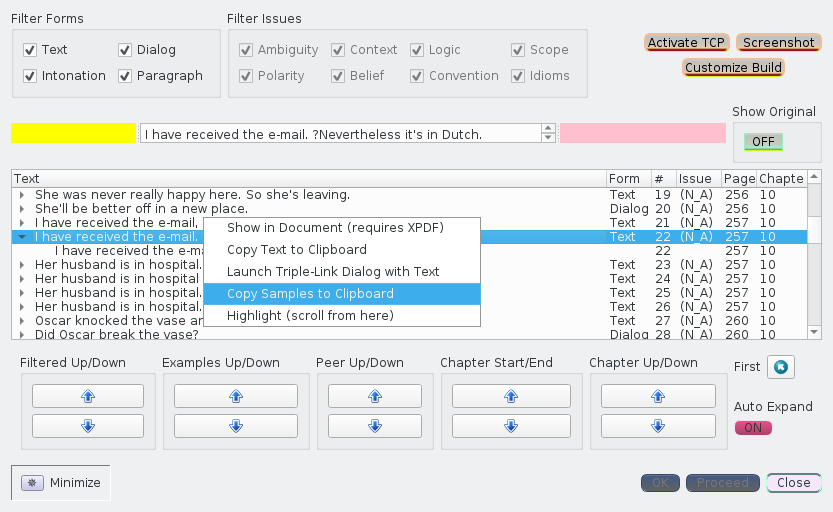
\includegraphics[scale=1.2]{texs/lingcopy.png}}
            
  \node [text width=10cm,inner sep=14pt,align=justify,fill=logoCyan!20, draw=logoBlue, 
  draw opacity=0.5,line width=1mm, fill opacity=0.9]
   at (0.29,0.82){\annfont\textbf{The linguistic samples comprising 
   this data set are all example sentences, phrases, 
   or dialog-snippets that are used, in the \textit{Blackwell 
   Handbook of Pragmatics}, as expository samples for 
   case-studies of various linguistic phenomenon and 
   pragmatics, semantics, and grammatical theories.}};
    
%notatedFigureBox{0.93,0.02}{0.985,0.945}{1}{0.985,0.945}%                
%\annotatedFigureBox{0.005,0.82}{0.43,0.98}{2}{0.43,0.82}%
%\annotatedFigureBox{0.01,0.1}{0.55,0.334}{3}{0.55,0.334}            
            
      %      \annotatedFigureBox{0.222,0.284}{0.3743,0.4934}{B}{0.3743,0.4934}%tr
      %      \annotatedFigureBox{0.555,0.784}{0.6815,0.874}{C}{0.555,0.784}%bl
      %      \annotatedFigureBox{0.557,0.322}{0.8985,0.5269}{D}{0.8985,0.5269}%tr
  

  
        \end{annotatedFigure}

\end{frame}


